\chapter{Working environment}
In section \ref{sec:vmclass} we introduced a classification of Virtual Machine systems.

The work presented in this thesis is restricted to same-ISA System Virtual Machines, where the Virtual Machine Monitor is a type 2 VMM.
In other words, we will deal with VMs that able to run an arbitrary OS compiled for the host ISA. The guest OS can in turn provide an 
execution environment for many user application.
Since the VMM is of type 2, it is implemented as a regular process in the host OS, and can make use of all the OS services.
We can therefore access the physical resource without requiring administrator previleges.

We also restrict our work to VMMs that make use of hardware-based virtualization, because the optimizations we will intrduce are
particularly effective in limiting the amount of VM switches between the host world and the guest world. Since these VM switches
are very expensive with hardware virtualization, the performance gain is significant.

While the assumptions made may appear restrictive, they are not at all. The class of VMMs that we consider is extremely 
common in the world of computing. They are used in datacenters and IT departments for server consolidation, 
application isolation, or to provide users/developers with zero-setup computing environments and other application in which it's
not important that the computing environment supported the VM has a different ISA from the host ISA.

\vspace{0.5cm}

Several VMM software belonging to the considered class are available. QEMU, VirtualBox, VMWare, Parallels, Windows
Hyper-V or Windows VirtualPC are among the most common examples of this kind of VMMs. These software tools are extremely widespread
and for this reason performance optimizations in these area are certainly useful.

This said, we have chosen the QEMU-KVM Virtual Machine Monitor for implementations and tests, although our optimizations are
relevant to the entire class of VMMs.

A GNU/Linux-based operating system (Archlinux) have been used on the host machine. The guest OS is generally Archlinux, but 
some tests have been performed with FreeBSD as a guest, too. Although Linux is a kernel and not a complete OS, in the following we 
will use  the expression ``Linux OS'' to actually mean ``GUN/Linux-based OS'', for the sake of simplicity.

\vspace{0.5cm}

Since our optimizations concern network performance, we had to choose a network device to work with. The \emph{e1000} class of 
network devices was chosen, since it is emulated by the vast majority of VMMs and supported by the main OSs (Windows, Linux, FreeBSD).


\section{QEMU features}
QEMU is a free, open source and multi-platform type 2 VMM, that makes use of dynamic translation to achieve good emulation performance.
QEMU-KVM is a QEMU branch that extends the original software to take advantage of hardware-based virtualization.
Whenever possible, QEMU-KVM uses hardware virtualization in order to execute guest code natively.
In the following we will use the terms QEMU and QEMU-KVM in an interchangeable manner.
At the date of this writing, the QEMU-KVM version number is 1.2.0, so we will refer to that version.

QEMU is a very flexible tool:
\begin{itemize}
    \item It supports process virtual machines: by means of dynamic translation it can execute on the host OS a single program compiled 
	  for an other ISA. This operating mode is called \emph{User mode emulation}.
	  
    \item It supports system virtual machines: by means of dynamic translation and hardware-assisted virtualization (when possible) it
	  can emulate full computer systems (including common peripherals), supporting unmodified operating systems. This operating
	  mode (which is the one we are interested in) is called \emph{Full system emulation}.
	  
    \item It supports various architectures, including  IA-32 (x86), x86-64, MIPS R4000, Sun's SPARC sun4m, Sun's SPARC sun4u,
	  ARM development boards (Integrator/CP and Versatile/PB), SH4 SHIX board, PowerPC,
	  ETRAX CRIS and MicroBlaze architectures.
	  
    \item It can emulate Symmetric Multiprocessing Systems (SMP), making use of all the CPUs that are present on the 
	  host system.
	  
    \item It is able to emulate various peripherals, such as hard disks, CD-ROM drives, network cards, audio interfaces, 
	  or USB devices.
	  
    \item Like similar hypervisors, it is able to provide its VM with network connectivity. The way this can be done will be
	  presented in section \ref{sec:qemunet}.
	  
    \item It does not normally require administrative rights to run. In our experiments administrative rights won't be
	  necessary.
\end{itemize}

QEMU is able to emulate the \emph{e1000} class of PCI network devices\footnote{To be more precise, the emulated hardware exposes
to the guest OS the PCI device ID of the 82540EM model.}, as well as other network devices (RTL8139C+, i8255x (PRO100), 
NE2000 (RTL8029), AMD PCNET II (Am79C7070a)).

In addition to that, QEMU support the \emph{Virtio} framework, that exposes a paravirtualized network device, virtio-net, intended 
to be used for high performance networking. The Virtio paravirtualized soution will be analized later.



\section{QEMU internal architecture}
In this section we will illustrate those details of QEMU implementation that are necessary to understand in order to reach our
goals.

\subsection{QEMU event-loop}
QEMU is an event-loop based software, and is implemented as a single-process multi-threaded application. 
One thread, referred to as \emph{IOThread}, executes the event-loop, waiting for new events to happen\footnote{This is 
implemented in \texttt{main-loop.c}}.
The waiting routine is a \texttt{select()} system call, which is not the most efficient choice on Unix-like systems
\footnote{ \texttt{poll()}, and espcially Linux \texttt{epoll()} or BSD \texttt{kqueue()} are more efficient},
but is more portable across different platforms.

\vspace{0.5cm}

The file descriptors associated with the \texttt{select()} can be associated to regular files, sockets, device files (such as TAP 
devices), or even special in-kernel objects, such as POSIX timers, signals and eventfds. These file descriptors are used by QEMU to let
the VM communicate with the host, and possibly with the rest of the Internet. In other words, they are used for performing the I/O 
operations requested by the VM. Of course the guest OS still performs I/O operations accessing I/O ports or memory-mapped I/O (MMIO) in 
his physical address space and is unaware of being emulated.

\vspace{0.5cm}

The QEMU core codebase offers to the QEMU developer an API that can be used to implement emulation of the devices.
The API also provides two useful abstractions: the QEMUTimer and the QEMUBH. 

QEMUTimers are a one-shot absolute timers, that can be 
used to execute a callback function at a certain point of time in the future. The callback is always executed by the IOThread, when it
recognizes that the deadline has been passed. The QEMUTimers are supported
by the Linux OS with a single one-shot relative POSIX timer\footnote{Similar mechanisms are used in other OS, or if POSIX timers are not
available under the Linux OS}, which is always (re)armed to expire - waking up the event-loop - at
the earliest deadline. The expire check for QEMUTimers is done at the end of each event-loop iteration, even if the event-loop was 
waken up for a reason different from the POSIX timer expiration. In the current implementation, moreover, every time the POSIX timer
is rearmed, the relative deadline is forced to be greater or equal that 250 $\mu$s\footnote{For more information about the QEMUTimer
interface and implementation, please refer to the file \texttt{qemu-timer.c} in the QEMU project root directory.}.

\vspace{0.5cm}

QEMUBH is the QEMU abstraction of the \emph{bottom half} concept, widely used in OS driver implementation. A QEMUBH can be seen as
a QEMUTimer that expires as soon as possible. In practice when a QEMUBH is scheduled, it notifies the event-loop, which in turn 
wakes up (or finishes the current iteration and begins another iteration) and execute all the callbacks of currently scheduled QEMUBHs.
Therefore the QEMUBH callbacks are always executed by the IOThread, similarly to the QEMUTimer callbacks\footnote{For more information
about the QEMUBH interface and implementation, please refer to the files \texttt{qemu-aio.h} and \texttt{async.c} in the QEMU project
root directory}. This feature is very important in terms of parallelism, as will be clear in the following chapters.

\subsection{VCPU Threads}
The IOThread, while executing the event-loop, handles all the interactions between the VM and the external world.
The guest code, however, is executed by one or more threads, that we will call \emph{VCPU threads}. In the current implementation QEMU
creates as many VCPU threads as the number of SMP processors specified by the users.
When using hardware-based virtualization (we made this assumption at the beginning of this chapter), a VCPU thread continuously
switch between the VM mode and the normal mode (see section \ref{sec:hbv}).

When the VCPU tries to execute an I/O operation - accessing I/O ports or MMIO - a VMExit happens. There could be other events
that cause a VMExit, but I/O operations are the type of events we are interested in. On a VMExit the VCPU stops executing guest
code and starts executing QEMU code, in order to handle - if is the case - the event that caused the VMExit.
When the event is handled, the VPCU executes e VMEnter and continues to run the guest code.

\vspace{0.5cm}

Since multiple threads are involved, and all of them - IOThread included - can access the shared structures used by the emulator
(e.g. the structures employed to implement the virtual devices), mutual exclusion is required. In the current implementation the
mutual exclusion is guaranteed by a single big-lock, called the \texttt{iothread lock}.

Therefore, on every VMExit a VCPU has to acquire the \texttt{iothread lock} before it can handle the event. After the event has been
handled, the VPCU thread release the \texttt{iothread lock} and execute a VMEnter instruction.
Similarly, the IOthread has to acquire the \texttt{iothread lock} every time it wakes up for event handling, and release the lock
only when the event-loop iteration terminates.

Putting all together, the figure \ref{fig:qemuthreads} depicts the QEMU thread scheme.

\begin{figure}[bt]
\centering
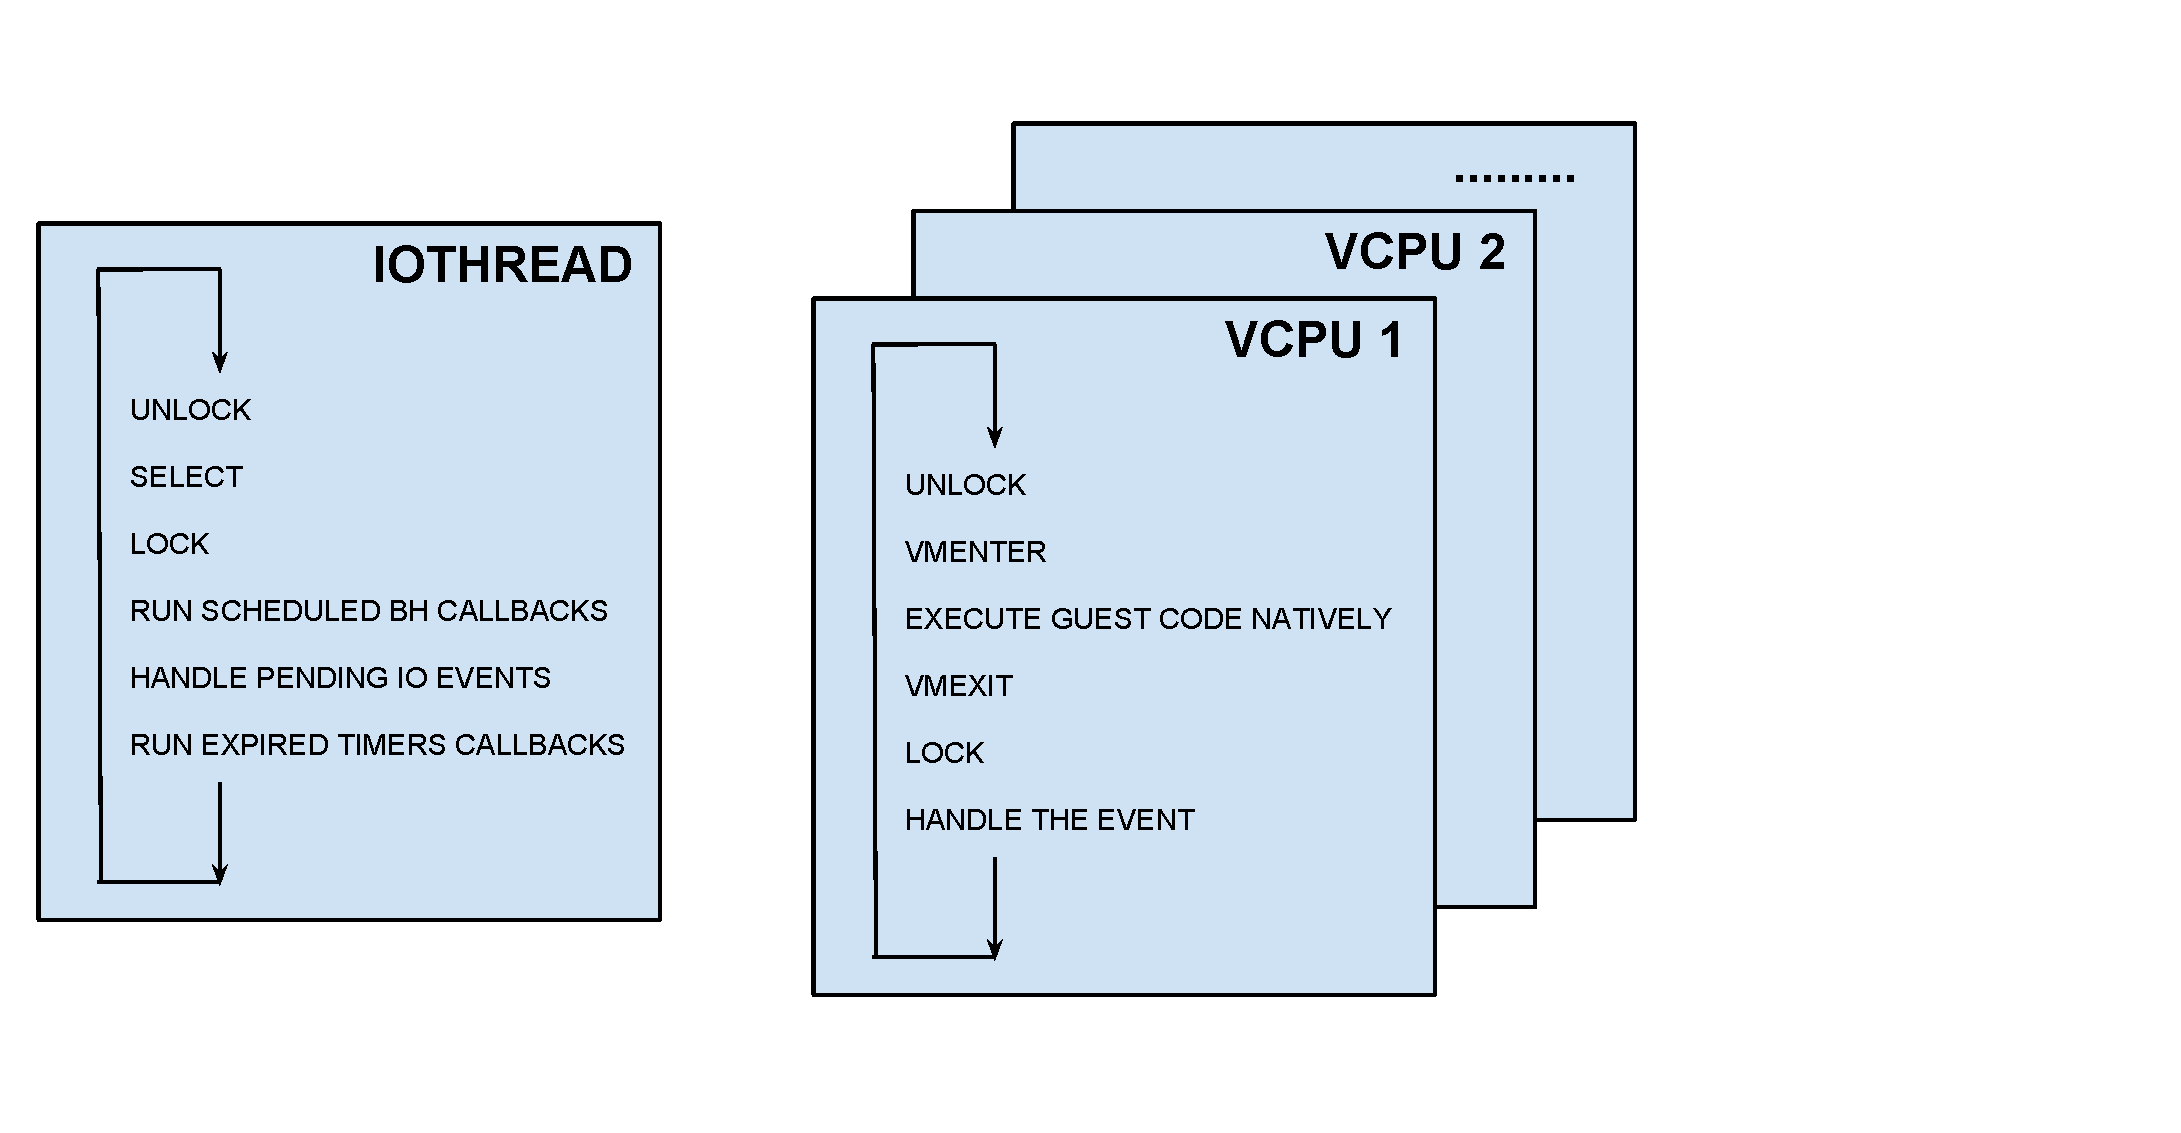
\includegraphics[scale = 0.45]{qemu-threads.pdf}
\caption{QEMU thread scheme.}
\label{fig:qemuthreads}
\end{figure}



\subsection{Network architectures}
\label{sec:qemunet}
When running a VM it is of fundamental importance to make possible for the guest to communicate with the outside world using the
networking infrastructure, otherwise the VM itself would be an useless computing box.

Since the VM it's a software entity, however, it isn't connected to any real network. Therefore the hypervisor has to provide some
form of network infrastructure virtualization, so that the guest OS thinks its (virtual) network device is connected to a physical
network and can then exchange packets with the outside.

\vspace{0.5cm}

All the hypervisors cited previously (QEMU included) provide the VM administrator with a few virtual network infrastructure modes, 
so that she can choose the best way to connect her VM.

Three modes are commonly employed:
\begin{itemize}
    \item NAT mode. In this case the guest OS thinks to be physically connected to a completely fake LAN, entirely emulated inside the 
	  hypervisor. The VMM usually emulates a DHCP server, a DNS server and a gateway router, so that the guest OS can configure
	  its network interfaces and its routing tables
	  and communicate with the outside world. When the guest sends a TCP/UDP packet on the fake LAN, the VMM intercepts the packet,
	  performs address translation (NAT) turning the guest source IP (the guest IP) into the host IP and sends the packet towards
	  its destination using the host OS services (thus the host OS routing tables). The inverse translation is performed when
	  receiving a packet.
	  
	  In this way the VM is easily provided with Internet connectivity, but it's not visible form the outside
	  and cannot communicate with other VMs present on the same host.
	  In QEMU this mode is called \emph{Usermode networking}.

    \item Host-only mode. Also in this case the guest OS thinks to be physically connected to a LAN. The LAN is emulated
	  by means of a software bridge (that emulates a layer-2 network switch), and the VM is connected to a port of the bridge.
	  More VMs can be connected to the same bridge, making inter-VM communication possible. The software bridge can be internally
	  implemented in the hypervisor, or can be an external software bridge.
	  
	  Whit QEMU this mode can be set up on a Linux host using the in-kernel bridging and TAP interfaces. Each VM is assigned a TAP
	  interface where can write/read ethernet frames, and all the TAPs are bridged together to the in-kernel bridge.
	  In this way a frame sent by the guest is written by QEMU to its associated TAP and is therefore routed by the bridge
	  to the correct destination TAP. The receiving QEMU process can then read the frame from the TAP and push it to its VM.
	  In this case no DHCP or DNS server is emulated, and you have to configure yourself the network of each VM\footnote{The 
	  configuration can be static or you can run a DHCP server on one of the VMs connected to the bridge.}.
	  Since the software bridge itself has its separate network interface, also the host can communicate on the LAN.
	  
    \item Bridged mode. This mode is an extension of the host-only mode. The only difference is that a physical host network interface
	  is also bridged to the VMs LAN. Since the physical interface becomes a bridge port, the host can access the physical network
	  through the software bridge interface.
	  In this way the host can share its connectivity with all the VM connected to the software bridge. If the physical interface
	  is connected to a LAN, with this configuration the VMs LAN appears to be part of the physical LAN.
	  
\end{itemize}
	
Clearly the NAT mode is not interesting with respect to our goals, since it is only a way the VM can easily obtain Internet 
connectivity, and it's not intended to be a flexible networking mode. Instead we will consider host-only mode, since we
are intersted in optimizing the communication performance between two VMs on the same software bridge or between a VM and the host
bridge interface. In this work it would make no sense considering to bridge also the host physical interfaces (bridged mode), 
because we optimizing performance of physical network adapter it's not among our goals.


\subsection{Network frontend and backend}
Déh, ci so' du peri.

%In our case the \emph{e1000} device is implemented through a single source file\footnote{hw/e1000.c in the QEMU project root directory}.
%A small part of this code contains declarations and routines necessary to register and initialize/uninitialize a new PCI Ethernet 
%device within the rest of the emulator. In this way one or more instances of the e1000 network device can be included by the QEMU users
%when launching QEMU\footnote{This is done through the \texttt{device} option. E.g. \texttt{qemu-kvm -device e1000 ...} }.




\section{The e1000 network adapter}
Vedi il manuale Intel.
